% =====================================================================
%  MSACL DS301 Deep Learning · Quiz 4 · Making Training Actually Work
%  Academic problem-set style (single-source, \ifsolution toggle)
%  SINGLE SOURCE — produces BOTH the student quiz and the answer key.
%
%  ANSWER TOGGLE
%  -------------
%  Student version (answers HIDDEN) — the default:
%       pdflatex quiz04_training_practice.tex
%  Answer key (answers SHOWN):
%       pdflatex "\def\showsolutions{}% =====================================================================
%  MSACL DS301 Deep Learning · Quiz 4 · Making Training Actually Work
%  Academic problem-set style (single-source, \ifsolution toggle)
%  SINGLE SOURCE — produces BOTH the student quiz and the answer key.
%
%  ANSWER TOGGLE
%  -------------
%  Student version (answers HIDDEN) — the default:
%       pdflatex quiz04_training_practice.tex
%  Answer key (answers SHOWN):
%       pdflatex "\def\showsolutions{}% =====================================================================
%  MSACL DS301 Deep Learning · Quiz 4 · Making Training Actually Work
%  Academic problem-set style (single-source, \ifsolution toggle)
%  SINGLE SOURCE — produces BOTH the student quiz and the answer key.
%
%  ANSWER TOGGLE
%  -------------
%  Student version (answers HIDDEN) — the default:
%       pdflatex quiz04_training_practice.tex
%  Answer key (answers SHOWN):
%       pdflatex "\def\showsolutions{}% =====================================================================
%  MSACL DS301 Deep Learning · Quiz 4 · Making Training Actually Work
%  Academic problem-set style (single-source, \ifsolution toggle)
%  SINGLE SOURCE — produces BOTH the student quiz and the answer key.
%
%  ANSWER TOGGLE
%  -------------
%  Student version (answers HIDDEN) — the default:
%       pdflatex quiz04_training_practice.tex
%  Answer key (answers SHOWN):
%       pdflatex "\def\showsolutions{}\input{quiz04_training_practice.tex}"
%  (or, to flip by hand, change \solutionfalse to \solutiontrue below.)
% =====================================================================
\documentclass[11pt]{article}

\newif\ifsolution
\ifdefined\showsolutions \solutiontrue \else \solutionfalse \fi
% \solutiontrue   % <-- uncomment to hard-code the ANSWER KEY build

\usepackage[letterpaper, margin=0.6in, top=0.7in, bottom=0.5in]{geometry}
\usepackage{amsmath, amssymb}
\usepackage{xcolor}
\usepackage{tikz}
\usepackage{fancyhdr}

\pagestyle{fancy}
\fancyhf{}
\fancyhead[L]{\small\textbf{MSACL DS301 --- Deep Learning}}
\fancyhead[R]{\small\textbf{Quiz 4: Making Training Actually Work\ifsolution\ \textmd{(Answer Key)}\fi}}
\fancyfoot[C]{\thepage}
\renewcommand{\headrulewidth}{0.4pt}

\newcommand{\blk}[1]{\underline{\hspace{#1}}}
% Reveal-or-blank: shows the answer in the key, a blank rule on the student sheet.
\newcommand{\rb}[2]{\ifsolution\textbf{#1}\else\blk{#2}\fi}
% Boxed answer (key only) and blank writing space (student only).
\newcommand{\keybox}[1]{\ifsolution\par\vspace{2pt}%
  \fbox{\parbox{0.965\textwidth}{\small\textbf{Answer.}\; #1}}\par\fi}
\newcommand{\work}[1]{\ifsolution\else\vspace{#1}\fi}

\setlength{\parindent}{0pt}
\setlength{\parskip}{3pt}
\setlength{\abovedisplayskip}{5pt}
\setlength{\belowdisplayskip}{5pt}

\begin{document}

\begin{center}
{\Large \textbf{Quiz 4 --- Making Training Actually Work}}\\[2pt]
{\normalsize Overfitting curves, the batch-size trade-off, and a discussion on class imbalance}
\end{center}

\vspace{-2pt}
\begin{center}
\fbox{\parbox{0.92\textwidth}{\small
\textbf{Instructions:}\; Answer all four questions --- the last two (Q3--Q4) are short
\emph{discussion} prompts on a topic we don't have lecture time to cover, so reason them out
in a sentence or two. Intuition first; no calculators needed.%
\ifsolution\else\\[4pt]\textbf{Name:}\ \blk{6cm}\hfill\textbf{Date:}\ \blk{3.5cm}\fi
}}
\end{center}

\vspace{-2pt}\hrule\vspace{5pt}

% =========================== Q1 ===========================
\textbf{1. Diagnose the training run --- and prescribe a fix.}\; {\small Each plot shows
\emph{training} loss (solid) and \emph{validation} loss (dashed) vs.\ epoch. For each, write the
\emph{diagnosis} and \emph{one fix}, using the word banks below.}

\vspace{4pt}
\begin{center}
\newcommand{\lossaxes}{\draw[->,gray] (0,0)--(3.1,0); \draw[->,gray] (0,0)--(0,2.5);}
%
\begin{minipage}[t]{0.235\linewidth}\centering

\begin{tikzpicture}[scale=0.8, line cap=round]
  \lossaxes
  % both high, close, flat -> underfit
  \draw[very thick] plot[smooth] coordinates {(0.15,2.15)(1.0,1.95)(2.0,1.85)(2.95,1.8)};
  \draw[very thick, dashed] plot[smooth] coordinates {(0.15,2.25)(1.0,2.05)(2.0,1.97)(2.95,1.92)};
\end{tikzpicture}\\[2pt]
{\footnotesize (a)}\\[3pt]
{\scriptsize diag:}\;\rb{underfitting}{1.5cm}\\[4pt]
{\scriptsize fix:}\;\rb{bigger/longer}{1.5cm}
\end{minipage}\hfill
%
\begin{minipage}[t]{0.235\linewidth}\centering
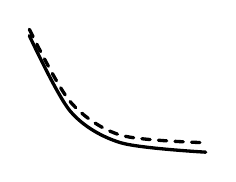
\begin{tikzpicture}[scale=0.8, line cap=round]
  \lossaxes
  % both drop low, small gap -> just right
  \draw[very thick] plot[smooth] coordinates {(0.15,2.2)(0.8,1.0)(1.6,0.5)(2.95,0.35)};
  \draw[very thick, dashed] plot[smooth] coordinates {(0.15,2.3)(0.8,1.15)(1.6,0.62)(2.95,0.5)};
\end{tikzpicture}\\[2pt]
{\footnotesize (b)}\\[3pt]
{\scriptsize diag:}\;\rb{just right}{1.5cm}\\[4pt]
{\scriptsize fix:}\;\rb{keep / ship it}{1.5cm}
\end{minipage}\hfill
%
\begin{minipage}[t]{0.235\linewidth}\centering
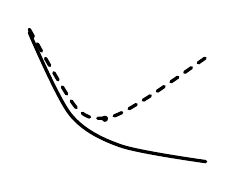
\begin{tikzpicture}[scale=0.8, line cap=round]
  \lossaxes
  % train keeps dropping, val dips then rises -> overfit
  \draw[very thick] plot[smooth] coordinates {(0.15,2.2)(0.8,0.9)(1.6,0.4)(2.95,0.15)};
  \draw[very thick, dashed] plot[smooth] coordinates {(0.15,2.25)(0.9,1.0)(1.4,0.85)(2.0,1.15)(2.95,1.8)};
  \fill[black] (1.35,0.83) circle (1.4pt);
\end{tikzpicture}\\[2pt]
{\footnotesize (c)}\\[3pt]
{\scriptsize diag:}\;\rb{overfitting}{1.5cm}\\[4pt]
{\scriptsize fix:}\;\rb{regularize}{1.5cm}
\end{minipage}\hfill
%
\begin{minipage}[t]{0.235\linewidth}\centering
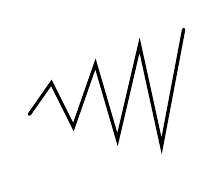
\begin{tikzpicture}[scale=0.8, line cap=round]
  \lossaxes
  % both diverge upward / jagged -> LR too high (not the same as a,c)
  \draw[very thick] (0.15,1.0)--(0.5,1.5)--(0.85,0.8)--(1.2,1.8)--(1.55,0.6)--(1.9,2.1)--(2.25,0.5)--(2.6,2.35);
\end{tikzpicture}\\[2pt]
{\footnotesize (d)}\\[3pt]
{\scriptsize diag:}\;\rb{LR too high}{1.5cm}\\[4pt]
{\scriptsize fix:}\;\rb{lower the LR}{1.5cm}
\end{minipage}
\end{center}

\vspace{2pt}
\begin{center}
{\small \textbf{Diagnosis bank:}\;\; underfitting \;$\cdot$\; just right \;$\cdot$\; overfitting
\;$\cdot$\; learning rate far too high (diverging) \\[2pt]
\textbf{Fix bank:}\;\; make the model bigger / train longer \;$\cdot$\; keep it (ship it)
\;$\cdot$\; regularize (dropout / weight decay / early stopping / more data) \;$\cdot$\;
lower the learning rate}
\end{center}

\keybox{(a) \textbf{underfitting $\rightarrow$ bigger model / train longer}: both curves sit high and
close and barely move --- the model is too weak or hasn't trained enough, so it hasn't even fit the
training data yet. (b) \textbf{just right $\rightarrow$ keep it}: both drop low and stay close, with
only a small gap --- validation tracks training down. (c) \textbf{overfitting $\rightarrow$
regularize}: training loss keeps falling toward zero while validation \emph{turns back up} (dot marks
the best epoch) --- the model is memorizing training quirks; add dropout / weight decay, stop early,
or get more/more-varied data. (d) \textbf{learning rate far too high $\rightarrow$ lower it}: the
(training) loss swings wildly and \emph{climbs} --- the steps are overshooting; this is a bad-LR
problem, not a capacity or memorizing problem. \emph{The tell for (c) vs.\ the rest: only in (c) do
the two curves \emph{split apart} --- training good, validation bad.}}

\vspace{2pt}\hrule\vspace{5pt}

% =========================== Q2 ===========================
\textbf{2. The batch-size trade-off.}\; {\small You are training a spectra classifier on Colab and
consider raising the mini-batch size from 32 to a much larger value.}

\vspace{3pt}
\textbf{(a)} Name \emph{one} thing a \emph{bigger} batch buys you.

\work{1.0cm}
\ifsolution\else\blk{\linewidth}\fi

\textbf{(b)} Name \emph{two} problems that appear if the batch is made \emph{too big}.

\work{1.4cm}
\ifsolution\else\blk{\linewidth}\\[10pt]\blk{\linewidth}\fi

\keybox{(a) A bigger batch gives a \textbf{less noisy, more reliable gradient estimate} (each step
points more accurately downhill) \emph{and/or} \textbf{better use of the GPU} (bulk matrix math is
efficient), so each step is steadier. \emph{Either is fine.}\\[3pt]
(b) Any \textbf{two} of: (i) \textbf{fewer weight updates per epoch} --- for a fixed number of
epochs you take far fewer steps, so learning per epoch stalls; (ii) it \textbf{may not fit in memory}
(a T4 will run out and crash); (iii) the very ``clean'' gradient tends to settle into
\textbf{sharp minima that generalize worse}, so accuracy on new samples can actually drop.
\emph{Practical rule: start around 32 and only grow it if training stays stable and validation
doesn't suffer.}}

\vspace{2pt}\hrule\vspace{5pt}

% =========================== Q3 (discussion) ===========================
\textbf{3. Discussion --- a rare but critical class.}\; {\small In a MALDI-TOF resistance panel,
only $5\%$ of isolates are \emph{resistant} (R); the other $95\%$ are \emph{susceptible} (S). You
train a classifier and it reports \textbf{95\% accuracy}.}

\vspace{3pt}
\textbf{(a)} Why might that 95\% accuracy be \emph{misleading} here --- what could the model be doing?

\work{1.0cm}
\ifsolution\else\blk{\linewidth}\fi

\textbf{(b)} What would you look at \emph{instead} of overall accuracy to know it actually catches the
resistant cases?

\work{1.2cm}
\ifsolution\else\blk{\linewidth}\fi

\keybox{(a) A model that simply \textbf{always predicts ``susceptible''} scores $95\%$ accuracy while
catching \emph{zero} resistant isolates --- with a rare class, overall accuracy is dominated by the
majority and can hide total failure on the cases that matter most. (b) Look at \textbf{class-specific}
measures: \textbf{sensitivity/recall on the resistant class} (what fraction of true R it catches),
\textbf{precision}, the \textbf{confusion matrix}, and a \textbf{precision--recall curve / PR-AUC}
--- not overall accuracy. (Sensitivity \& specificity return in Lecture 10.)}

\vspace{2pt}\hrule\vspace{5pt}

% =========================== Q4 (discussion) ===========================
\textbf{4. Discussion --- what would you try?}\; {\small Same imbalanced problem. Name \emph{two}
things you could do so the model pays real attention to the rare resistant class. (One line each.)}

\work{1.4cm}
\ifsolution\else\blk{\linewidth}\\[10pt]\blk{\linewidth}\fi

\keybox{Any \textbf{two} reasonable ideas, e.g.: \textbf{get or oversample more resistant examples}
(or augment them); \textbf{undersample} the susceptible majority; \textbf{weight the loss} toward the
rare class (class weights) or use \textbf{focal loss} to turn up the rare/hard cases; \textbf{move the
decision threshold} to favour catching R; \textbf{choose metrics} (sensitivity, precision--recall)
that reflect the real goal; use \textbf{stratified} train/validation splits. (All revisited in
Lecture 10 --- this prompt just gets them thinking.)}

\vspace{4pt}\hrule\vspace{3pt}
{\small\itshape \ifsolution Answer key.\else Keep this sheet --- the overfitting fixes and the
batch-size rule of thumb are your Lab 2 cheat-sheet.\fi}

\end{document}
"
%  (or, to flip by hand, change \solutionfalse to \solutiontrue below.)
% =====================================================================
\documentclass[11pt]{article}

\newif\ifsolution
\ifdefined\showsolutions \solutiontrue \else \solutionfalse \fi
% \solutiontrue   % <-- uncomment to hard-code the ANSWER KEY build

\usepackage[letterpaper, margin=0.6in, top=0.7in, bottom=0.5in]{geometry}
\usepackage{amsmath, amssymb}
\usepackage{xcolor}
\usepackage{tikz}
\usepackage{fancyhdr}

\pagestyle{fancy}
\fancyhf{}
\fancyhead[L]{\small\textbf{MSACL DS301 --- Deep Learning}}
\fancyhead[R]{\small\textbf{Quiz 4: Making Training Actually Work\ifsolution\ \textmd{(Answer Key)}\fi}}
\fancyfoot[C]{\thepage}
\renewcommand{\headrulewidth}{0.4pt}

\newcommand{\blk}[1]{\underline{\hspace{#1}}}
% Reveal-or-blank: shows the answer in the key, a blank rule on the student sheet.
\newcommand{\rb}[2]{\ifsolution\textbf{#1}\else\blk{#2}\fi}
% Boxed answer (key only) and blank writing space (student only).
\newcommand{\keybox}[1]{\ifsolution\par\vspace{2pt}%
  \fbox{\parbox{0.965\textwidth}{\small\textbf{Answer.}\; #1}}\par\fi}
\newcommand{\work}[1]{\ifsolution\else\vspace{#1}\fi}

\setlength{\parindent}{0pt}
\setlength{\parskip}{3pt}
\setlength{\abovedisplayskip}{5pt}
\setlength{\belowdisplayskip}{5pt}

\begin{document}

\begin{center}
{\Large \textbf{Quiz 4 --- Making Training Actually Work}}\\[2pt]
{\normalsize Overfitting curves, the batch-size trade-off, and a discussion on class imbalance}
\end{center}

\vspace{-2pt}
\begin{center}
\fbox{\parbox{0.92\textwidth}{\small
\textbf{Instructions:}\; Answer all four questions --- the last two (Q3--Q4) are short
\emph{discussion} prompts on a topic we don't have lecture time to cover, so reason them out
in a sentence or two. Intuition first; no calculators needed.%
\ifsolution\else\\[4pt]\textbf{Name:}\ \blk{6cm}\hfill\textbf{Date:}\ \blk{3.5cm}\fi
}}
\end{center}

\vspace{-2pt}\hrule\vspace{5pt}

% =========================== Q1 ===========================
\textbf{1. Diagnose the training run --- and prescribe a fix.}\; {\small Each plot shows
\emph{training} loss (solid) and \emph{validation} loss (dashed) vs.\ epoch. For each, write the
\emph{diagnosis} and \emph{one fix}, using the word banks below.}

\vspace{4pt}
\begin{center}
\newcommand{\lossaxes}{\draw[->,gray] (0,0)--(3.1,0); \draw[->,gray] (0,0)--(0,2.5);}
%
\begin{minipage}[t]{0.235\linewidth}\centering

\begin{tikzpicture}[scale=0.8, line cap=round]
  \lossaxes
  % both high, close, flat -> underfit
  \draw[very thick] plot[smooth] coordinates {(0.15,2.15)(1.0,1.95)(2.0,1.85)(2.95,1.8)};
  \draw[very thick, dashed] plot[smooth] coordinates {(0.15,2.25)(1.0,2.05)(2.0,1.97)(2.95,1.92)};
\end{tikzpicture}\\[2pt]
{\footnotesize (a)}\\[3pt]
{\scriptsize diag:}\;\rb{underfitting}{1.5cm}\\[4pt]
{\scriptsize fix:}\;\rb{bigger/longer}{1.5cm}
\end{minipage}\hfill
%
\begin{minipage}[t]{0.235\linewidth}\centering
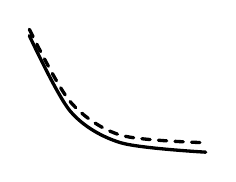
\begin{tikzpicture}[scale=0.8, line cap=round]
  \lossaxes
  % both drop low, small gap -> just right
  \draw[very thick] plot[smooth] coordinates {(0.15,2.2)(0.8,1.0)(1.6,0.5)(2.95,0.35)};
  \draw[very thick, dashed] plot[smooth] coordinates {(0.15,2.3)(0.8,1.15)(1.6,0.62)(2.95,0.5)};
\end{tikzpicture}\\[2pt]
{\footnotesize (b)}\\[3pt]
{\scriptsize diag:}\;\rb{just right}{1.5cm}\\[4pt]
{\scriptsize fix:}\;\rb{keep / ship it}{1.5cm}
\end{minipage}\hfill
%
\begin{minipage}[t]{0.235\linewidth}\centering
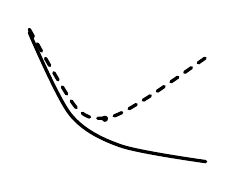
\begin{tikzpicture}[scale=0.8, line cap=round]
  \lossaxes
  % train keeps dropping, val dips then rises -> overfit
  \draw[very thick] plot[smooth] coordinates {(0.15,2.2)(0.8,0.9)(1.6,0.4)(2.95,0.15)};
  \draw[very thick, dashed] plot[smooth] coordinates {(0.15,2.25)(0.9,1.0)(1.4,0.85)(2.0,1.15)(2.95,1.8)};
  \fill[black] (1.35,0.83) circle (1.4pt);
\end{tikzpicture}\\[2pt]
{\footnotesize (c)}\\[3pt]
{\scriptsize diag:}\;\rb{overfitting}{1.5cm}\\[4pt]
{\scriptsize fix:}\;\rb{regularize}{1.5cm}
\end{minipage}\hfill
%
\begin{minipage}[t]{0.235\linewidth}\centering
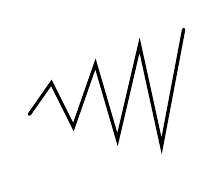
\begin{tikzpicture}[scale=0.8, line cap=round]
  \lossaxes
  % both diverge upward / jagged -> LR too high (not the same as a,c)
  \draw[very thick] (0.15,1.0)--(0.5,1.5)--(0.85,0.8)--(1.2,1.8)--(1.55,0.6)--(1.9,2.1)--(2.25,0.5)--(2.6,2.35);
\end{tikzpicture}\\[2pt]
{\footnotesize (d)}\\[3pt]
{\scriptsize diag:}\;\rb{LR too high}{1.5cm}\\[4pt]
{\scriptsize fix:}\;\rb{lower the LR}{1.5cm}
\end{minipage}
\end{center}

\vspace{2pt}
\begin{center}
{\small \textbf{Diagnosis bank:}\;\; underfitting \;$\cdot$\; just right \;$\cdot$\; overfitting
\;$\cdot$\; learning rate far too high (diverging) \\[2pt]
\textbf{Fix bank:}\;\; make the model bigger / train longer \;$\cdot$\; keep it (ship it)
\;$\cdot$\; regularize (dropout / weight decay / early stopping / more data) \;$\cdot$\;
lower the learning rate}
\end{center}

\keybox{(a) \textbf{underfitting $\rightarrow$ bigger model / train longer}: both curves sit high and
close and barely move --- the model is too weak or hasn't trained enough, so it hasn't even fit the
training data yet. (b) \textbf{just right $\rightarrow$ keep it}: both drop low and stay close, with
only a small gap --- validation tracks training down. (c) \textbf{overfitting $\rightarrow$
regularize}: training loss keeps falling toward zero while validation \emph{turns back up} (dot marks
the best epoch) --- the model is memorizing training quirks; add dropout / weight decay, stop early,
or get more/more-varied data. (d) \textbf{learning rate far too high $\rightarrow$ lower it}: the
(training) loss swings wildly and \emph{climbs} --- the steps are overshooting; this is a bad-LR
problem, not a capacity or memorizing problem. \emph{The tell for (c) vs.\ the rest: only in (c) do
the two curves \emph{split apart} --- training good, validation bad.}}

\vspace{2pt}\hrule\vspace{5pt}

% =========================== Q2 ===========================
\textbf{2. The batch-size trade-off.}\; {\small You are training a spectra classifier on Colab and
consider raising the mini-batch size from 32 to a much larger value.}

\vspace{3pt}
\textbf{(a)} Name \emph{one} thing a \emph{bigger} batch buys you.

\work{1.0cm}
\ifsolution\else\blk{\linewidth}\fi

\textbf{(b)} Name \emph{two} problems that appear if the batch is made \emph{too big}.

\work{1.4cm}
\ifsolution\else\blk{\linewidth}\\[10pt]\blk{\linewidth}\fi

\keybox{(a) A bigger batch gives a \textbf{less noisy, more reliable gradient estimate} (each step
points more accurately downhill) \emph{and/or} \textbf{better use of the GPU} (bulk matrix math is
efficient), so each step is steadier. \emph{Either is fine.}\\[3pt]
(b) Any \textbf{two} of: (i) \textbf{fewer weight updates per epoch} --- for a fixed number of
epochs you take far fewer steps, so learning per epoch stalls; (ii) it \textbf{may not fit in memory}
(a T4 will run out and crash); (iii) the very ``clean'' gradient tends to settle into
\textbf{sharp minima that generalize worse}, so accuracy on new samples can actually drop.
\emph{Practical rule: start around 32 and only grow it if training stays stable and validation
doesn't suffer.}}

\vspace{2pt}\hrule\vspace{5pt}

% =========================== Q3 (discussion) ===========================
\textbf{3. Discussion --- a rare but critical class.}\; {\small In a MALDI-TOF resistance panel,
only $5\%$ of isolates are \emph{resistant} (R); the other $95\%$ are \emph{susceptible} (S). You
train a classifier and it reports \textbf{95\% accuracy}.}

\vspace{3pt}
\textbf{(a)} Why might that 95\% accuracy be \emph{misleading} here --- what could the model be doing?

\work{1.0cm}
\ifsolution\else\blk{\linewidth}\fi

\textbf{(b)} What would you look at \emph{instead} of overall accuracy to know it actually catches the
resistant cases?

\work{1.2cm}
\ifsolution\else\blk{\linewidth}\fi

\keybox{(a) A model that simply \textbf{always predicts ``susceptible''} scores $95\%$ accuracy while
catching \emph{zero} resistant isolates --- with a rare class, overall accuracy is dominated by the
majority and can hide total failure on the cases that matter most. (b) Look at \textbf{class-specific}
measures: \textbf{sensitivity/recall on the resistant class} (what fraction of true R it catches),
\textbf{precision}, the \textbf{confusion matrix}, and a \textbf{precision--recall curve / PR-AUC}
--- not overall accuracy. (Sensitivity \& specificity return in Lecture 10.)}

\vspace{2pt}\hrule\vspace{5pt}

% =========================== Q4 (discussion) ===========================
\textbf{4. Discussion --- what would you try?}\; {\small Same imbalanced problem. Name \emph{two}
things you could do so the model pays real attention to the rare resistant class. (One line each.)}

\work{1.4cm}
\ifsolution\else\blk{\linewidth}\\[10pt]\blk{\linewidth}\fi

\keybox{Any \textbf{two} reasonable ideas, e.g.: \textbf{get or oversample more resistant examples}
(or augment them); \textbf{undersample} the susceptible majority; \textbf{weight the loss} toward the
rare class (class weights) or use \textbf{focal loss} to turn up the rare/hard cases; \textbf{move the
decision threshold} to favour catching R; \textbf{choose metrics} (sensitivity, precision--recall)
that reflect the real goal; use \textbf{stratified} train/validation splits. (All revisited in
Lecture 10 --- this prompt just gets them thinking.)}

\vspace{4pt}\hrule\vspace{3pt}
{\small\itshape \ifsolution Answer key.\else Keep this sheet --- the overfitting fixes and the
batch-size rule of thumb are your Lab 2 cheat-sheet.\fi}

\end{document}
"
%  (or, to flip by hand, change \solutionfalse to \solutiontrue below.)
% =====================================================================
\documentclass[11pt]{article}

\newif\ifsolution
\ifdefined\showsolutions \solutiontrue \else \solutionfalse \fi
% \solutiontrue   % <-- uncomment to hard-code the ANSWER KEY build

\usepackage[letterpaper, margin=0.6in, top=0.7in, bottom=0.5in]{geometry}
\usepackage{amsmath, amssymb}
\usepackage{xcolor}
\usepackage{tikz}
\usepackage{fancyhdr}

\pagestyle{fancy}
\fancyhf{}
\fancyhead[L]{\small\textbf{MSACL DS301 --- Deep Learning}}
\fancyhead[R]{\small\textbf{Quiz 4: Making Training Actually Work\ifsolution\ \textmd{(Answer Key)}\fi}}
\fancyfoot[C]{\thepage}
\renewcommand{\headrulewidth}{0.4pt}

\newcommand{\blk}[1]{\underline{\hspace{#1}}}
% Reveal-or-blank: shows the answer in the key, a blank rule on the student sheet.
\newcommand{\rb}[2]{\ifsolution\textbf{#1}\else\blk{#2}\fi}
% Boxed answer (key only) and blank writing space (student only).
\newcommand{\keybox}[1]{\ifsolution\par\vspace{2pt}%
  \fbox{\parbox{0.965\textwidth}{\small\textbf{Answer.}\; #1}}\par\fi}
\newcommand{\work}[1]{\ifsolution\else\vspace{#1}\fi}

\setlength{\parindent}{0pt}
\setlength{\parskip}{3pt}
\setlength{\abovedisplayskip}{5pt}
\setlength{\belowdisplayskip}{5pt}

\begin{document}

\begin{center}
{\Large \textbf{Quiz 4 --- Making Training Actually Work}}\\[2pt]
{\normalsize Overfitting curves, the batch-size trade-off, and a discussion on class imbalance}
\end{center}

\vspace{-2pt}
\begin{center}
\fbox{\parbox{0.92\textwidth}{\small
\textbf{Instructions:}\; Answer all four questions --- the last two (Q3--Q4) are short
\emph{discussion} prompts on a topic we don't have lecture time to cover, so reason them out
in a sentence or two. Intuition first; no calculators needed.%
\ifsolution\else\\[4pt]\textbf{Name:}\ \blk{6cm}\hfill\textbf{Date:}\ \blk{3.5cm}\fi
}}
\end{center}

\vspace{-2pt}\hrule\vspace{5pt}

% =========================== Q1 ===========================
\textbf{1. Diagnose the training run --- and prescribe a fix.}\; {\small Each plot shows
\emph{training} loss (solid) and \emph{validation} loss (dashed) vs.\ epoch. For each, write the
\emph{diagnosis} and \emph{one fix}, using the word banks below.}

\vspace{4pt}
\begin{center}
\newcommand{\lossaxes}{\draw[->,gray] (0,0)--(3.1,0); \draw[->,gray] (0,0)--(0,2.5);}
%
\begin{minipage}[t]{0.235\linewidth}\centering

\begin{tikzpicture}[scale=0.8, line cap=round]
  \lossaxes
  % both high, close, flat -> underfit
  \draw[very thick] plot[smooth] coordinates {(0.15,2.15)(1.0,1.95)(2.0,1.85)(2.95,1.8)};
  \draw[very thick, dashed] plot[smooth] coordinates {(0.15,2.25)(1.0,2.05)(2.0,1.97)(2.95,1.92)};
\end{tikzpicture}\\[2pt]
{\footnotesize (a)}\\[3pt]
{\scriptsize diag:}\;\rb{underfitting}{1.5cm}\\[4pt]
{\scriptsize fix:}\;\rb{bigger/longer}{1.5cm}
\end{minipage}\hfill
%
\begin{minipage}[t]{0.235\linewidth}\centering
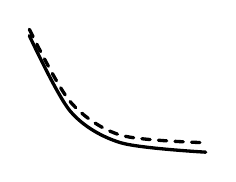
\begin{tikzpicture}[scale=0.8, line cap=round]
  \lossaxes
  % both drop low, small gap -> just right
  \draw[very thick] plot[smooth] coordinates {(0.15,2.2)(0.8,1.0)(1.6,0.5)(2.95,0.35)};
  \draw[very thick, dashed] plot[smooth] coordinates {(0.15,2.3)(0.8,1.15)(1.6,0.62)(2.95,0.5)};
\end{tikzpicture}\\[2pt]
{\footnotesize (b)}\\[3pt]
{\scriptsize diag:}\;\rb{just right}{1.5cm}\\[4pt]
{\scriptsize fix:}\;\rb{keep / ship it}{1.5cm}
\end{minipage}\hfill
%
\begin{minipage}[t]{0.235\linewidth}\centering
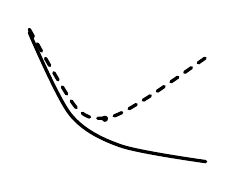
\begin{tikzpicture}[scale=0.8, line cap=round]
  \lossaxes
  % train keeps dropping, val dips then rises -> overfit
  \draw[very thick] plot[smooth] coordinates {(0.15,2.2)(0.8,0.9)(1.6,0.4)(2.95,0.15)};
  \draw[very thick, dashed] plot[smooth] coordinates {(0.15,2.25)(0.9,1.0)(1.4,0.85)(2.0,1.15)(2.95,1.8)};
  \fill[black] (1.35,0.83) circle (1.4pt);
\end{tikzpicture}\\[2pt]
{\footnotesize (c)}\\[3pt]
{\scriptsize diag:}\;\rb{overfitting}{1.5cm}\\[4pt]
{\scriptsize fix:}\;\rb{regularize}{1.5cm}
\end{minipage}\hfill
%
\begin{minipage}[t]{0.235\linewidth}\centering
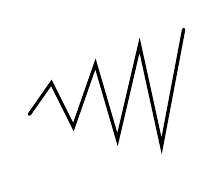
\begin{tikzpicture}[scale=0.8, line cap=round]
  \lossaxes
  % both diverge upward / jagged -> LR too high (not the same as a,c)
  \draw[very thick] (0.15,1.0)--(0.5,1.5)--(0.85,0.8)--(1.2,1.8)--(1.55,0.6)--(1.9,2.1)--(2.25,0.5)--(2.6,2.35);
\end{tikzpicture}\\[2pt]
{\footnotesize (d)}\\[3pt]
{\scriptsize diag:}\;\rb{LR too high}{1.5cm}\\[4pt]
{\scriptsize fix:}\;\rb{lower the LR}{1.5cm}
\end{minipage}
\end{center}

\vspace{2pt}
\begin{center}
{\small \textbf{Diagnosis bank:}\;\; underfitting \;$\cdot$\; just right \;$\cdot$\; overfitting
\;$\cdot$\; learning rate far too high (diverging) \\[2pt]
\textbf{Fix bank:}\;\; make the model bigger / train longer \;$\cdot$\; keep it (ship it)
\;$\cdot$\; regularize (dropout / weight decay / early stopping / more data) \;$\cdot$\;
lower the learning rate}
\end{center}

\keybox{(a) \textbf{underfitting $\rightarrow$ bigger model / train longer}: both curves sit high and
close and barely move --- the model is too weak or hasn't trained enough, so it hasn't even fit the
training data yet. (b) \textbf{just right $\rightarrow$ keep it}: both drop low and stay close, with
only a small gap --- validation tracks training down. (c) \textbf{overfitting $\rightarrow$
regularize}: training loss keeps falling toward zero while validation \emph{turns back up} (dot marks
the best epoch) --- the model is memorizing training quirks; add dropout / weight decay, stop early,
or get more/more-varied data. (d) \textbf{learning rate far too high $\rightarrow$ lower it}: the
(training) loss swings wildly and \emph{climbs} --- the steps are overshooting; this is a bad-LR
problem, not a capacity or memorizing problem. \emph{The tell for (c) vs.\ the rest: only in (c) do
the two curves \emph{split apart} --- training good, validation bad.}}

\vspace{2pt}\hrule\vspace{5pt}

% =========================== Q2 ===========================
\textbf{2. The batch-size trade-off.}\; {\small You are training a spectra classifier on Colab and
consider raising the mini-batch size from 32 to a much larger value.}

\vspace{3pt}
\textbf{(a)} Name \emph{one} thing a \emph{bigger} batch buys you.

\work{1.0cm}
\ifsolution\else\blk{\linewidth}\fi

\textbf{(b)} Name \emph{two} problems that appear if the batch is made \emph{too big}.

\work{1.4cm}
\ifsolution\else\blk{\linewidth}\\[10pt]\blk{\linewidth}\fi

\keybox{(a) A bigger batch gives a \textbf{less noisy, more reliable gradient estimate} (each step
points more accurately downhill) \emph{and/or} \textbf{better use of the GPU} (bulk matrix math is
efficient), so each step is steadier. \emph{Either is fine.}\\[3pt]
(b) Any \textbf{two} of: (i) \textbf{fewer weight updates per epoch} --- for a fixed number of
epochs you take far fewer steps, so learning per epoch stalls; (ii) it \textbf{may not fit in memory}
(a T4 will run out and crash); (iii) the very ``clean'' gradient tends to settle into
\textbf{sharp minima that generalize worse}, so accuracy on new samples can actually drop.
\emph{Practical rule: start around 32 and only grow it if training stays stable and validation
doesn't suffer.}}

\vspace{2pt}\hrule\vspace{5pt}

% =========================== Q3 (discussion) ===========================
\textbf{3. Discussion --- a rare but critical class.}\; {\small In a MALDI-TOF resistance panel,
only $5\%$ of isolates are \emph{resistant} (R); the other $95\%$ are \emph{susceptible} (S). You
train a classifier and it reports \textbf{95\% accuracy}.}

\vspace{3pt}
\textbf{(a)} Why might that 95\% accuracy be \emph{misleading} here --- what could the model be doing?

\work{1.0cm}
\ifsolution\else\blk{\linewidth}\fi

\textbf{(b)} What would you look at \emph{instead} of overall accuracy to know it actually catches the
resistant cases?

\work{1.2cm}
\ifsolution\else\blk{\linewidth}\fi

\keybox{(a) A model that simply \textbf{always predicts ``susceptible''} scores $95\%$ accuracy while
catching \emph{zero} resistant isolates --- with a rare class, overall accuracy is dominated by the
majority and can hide total failure on the cases that matter most. (b) Look at \textbf{class-specific}
measures: \textbf{sensitivity/recall on the resistant class} (what fraction of true R it catches),
\textbf{precision}, the \textbf{confusion matrix}, and a \textbf{precision--recall curve / PR-AUC}
--- not overall accuracy. (Sensitivity \& specificity return in Lecture 10.)}

\vspace{2pt}\hrule\vspace{5pt}

% =========================== Q4 (discussion) ===========================
\textbf{4. Discussion --- what would you try?}\; {\small Same imbalanced problem. Name \emph{two}
things you could do so the model pays real attention to the rare resistant class. (One line each.)}

\work{1.4cm}
\ifsolution\else\blk{\linewidth}\\[10pt]\blk{\linewidth}\fi

\keybox{Any \textbf{two} reasonable ideas, e.g.: \textbf{get or oversample more resistant examples}
(or augment them); \textbf{undersample} the susceptible majority; \textbf{weight the loss} toward the
rare class (class weights) or use \textbf{focal loss} to turn up the rare/hard cases; \textbf{move the
decision threshold} to favour catching R; \textbf{choose metrics} (sensitivity, precision--recall)
that reflect the real goal; use \textbf{stratified} train/validation splits. (All revisited in
Lecture 10 --- this prompt just gets them thinking.)}

\vspace{4pt}\hrule\vspace{3pt}
{\small\itshape \ifsolution Answer key.\else Keep this sheet --- the overfitting fixes and the
batch-size rule of thumb are your Lab 2 cheat-sheet.\fi}

\end{document}
"
%  (or, to flip by hand, change \solutionfalse to \solutiontrue below.)
% =====================================================================
\documentclass[11pt]{article}

\newif\ifsolution
\ifdefined\showsolutions \solutiontrue \else \solutionfalse \fi
% \solutiontrue   % <-- uncomment to hard-code the ANSWER KEY build

\usepackage[letterpaper, margin=0.6in, top=0.7in, bottom=0.5in]{geometry}
\usepackage{amsmath, amssymb}
\usepackage{xcolor}
\usepackage{tikz}
\usepackage{fancyhdr}

\pagestyle{fancy}
\fancyhf{}
\fancyhead[L]{\small\textbf{MSACL DS301 --- Deep Learning}}
\fancyhead[R]{\small\textbf{Quiz 4: Making Training Actually Work\ifsolution\ \textmd{(Answer Key)}\fi}}
\fancyfoot[C]{\thepage}
\renewcommand{\headrulewidth}{0.4pt}

\newcommand{\blk}[1]{\underline{\hspace{#1}}}
% Reveal-or-blank: shows the answer in the key, a blank rule on the student sheet.
\newcommand{\rb}[2]{\ifsolution\textbf{#1}\else\blk{#2}\fi}
% Boxed answer (key only) and blank writing space (student only).
\newcommand{\keybox}[1]{\ifsolution\par\vspace{2pt}%
  \fbox{\parbox{0.965\textwidth}{\small\textbf{Answer.}\; #1}}\par\fi}
\newcommand{\work}[1]{\ifsolution\else\vspace{#1}\fi}

\setlength{\parindent}{0pt}
\setlength{\parskip}{3pt}
\setlength{\abovedisplayskip}{5pt}
\setlength{\belowdisplayskip}{5pt}

\begin{document}

\begin{center}
{\Large \textbf{Quiz 4 --- Making Training Actually Work}}\\[2pt]
{\normalsize Overfitting curves, the batch-size trade-off, and a discussion on class imbalance}
\end{center}

\vspace{-2pt}
\begin{center}
\fbox{\parbox{0.92\textwidth}{\small
\textbf{Instructions:}\; Answer all four questions --- the last two (Q3--Q4) are short
\emph{discussion} prompts on a topic we don't have lecture time to cover, so reason them out
in a sentence or two. Intuition first; no calculators needed.%
\ifsolution\else\\[4pt]\textbf{Name:}\ \blk{6cm}\hfill\textbf{Date:}\ \blk{3.5cm}\fi
}}
\end{center}

\vspace{-2pt}\hrule\vspace{5pt}

% =========================== Q1 ===========================
\textbf{1. Diagnose the training run --- and prescribe a fix.}\; {\small Each plot shows
\emph{training} loss (solid) and \emph{validation} loss (dashed) vs.\ epoch. For each, write the
\emph{diagnosis} and \emph{one fix}, using the word banks below.}

\vspace{4pt}
\begin{center}
\newcommand{\lossaxes}{\draw[->,gray] (0,0)--(3.1,0); \draw[->,gray] (0,0)--(0,2.5);}
%
\begin{minipage}[t]{0.235\linewidth}\centering

\begin{tikzpicture}[scale=0.8, line cap=round]
  \lossaxes
  % both high, close, flat -> underfit
  \draw[very thick] plot[smooth] coordinates {(0.15,2.15)(1.0,1.95)(2.0,1.85)(2.95,1.8)};
  \draw[very thick, dashed] plot[smooth] coordinates {(0.15,2.25)(1.0,2.05)(2.0,1.97)(2.95,1.92)};
\end{tikzpicture}\\[2pt]
{\footnotesize (a)}\\[3pt]
{\scriptsize diag:}\;\rb{underfitting}{1.5cm}\\[4pt]
{\scriptsize fix:}\;\rb{bigger/longer}{1.5cm}
\end{minipage}\hfill
%
\begin{minipage}[t]{0.235\linewidth}\centering
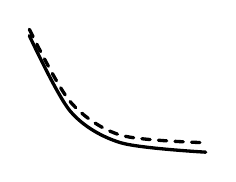
\begin{tikzpicture}[scale=0.8, line cap=round]
  \lossaxes
  % both drop low, small gap -> just right
  \draw[very thick] plot[smooth] coordinates {(0.15,2.2)(0.8,1.0)(1.6,0.5)(2.95,0.35)};
  \draw[very thick, dashed] plot[smooth] coordinates {(0.15,2.3)(0.8,1.15)(1.6,0.62)(2.95,0.5)};
\end{tikzpicture}\\[2pt]
{\footnotesize (b)}\\[3pt]
{\scriptsize diag:}\;\rb{just right}{1.5cm}\\[4pt]
{\scriptsize fix:}\;\rb{keep / ship it}{1.5cm}
\end{minipage}\hfill
%
\begin{minipage}[t]{0.235\linewidth}\centering
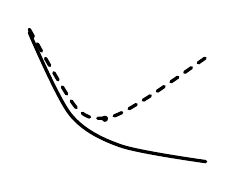
\begin{tikzpicture}[scale=0.8, line cap=round]
  \lossaxes
  % train keeps dropping, val dips then rises -> overfit
  \draw[very thick] plot[smooth] coordinates {(0.15,2.2)(0.8,0.9)(1.6,0.4)(2.95,0.15)};
  \draw[very thick, dashed] plot[smooth] coordinates {(0.15,2.25)(0.9,1.0)(1.4,0.85)(2.0,1.15)(2.95,1.8)};
  \fill[black] (1.35,0.83) circle (1.4pt);
\end{tikzpicture}\\[2pt]
{\footnotesize (c)}\\[3pt]
{\scriptsize diag:}\;\rb{overfitting}{1.5cm}\\[4pt]
{\scriptsize fix:}\;\rb{regularize}{1.5cm}
\end{minipage}\hfill
%
\begin{minipage}[t]{0.235\linewidth}\centering
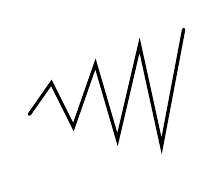
\begin{tikzpicture}[scale=0.8, line cap=round]
  \lossaxes
  % both diverge upward / jagged -> LR too high (not the same as a,c)
  \draw[very thick] (0.15,1.0)--(0.5,1.5)--(0.85,0.8)--(1.2,1.8)--(1.55,0.6)--(1.9,2.1)--(2.25,0.5)--(2.6,2.35);
\end{tikzpicture}\\[2pt]
{\footnotesize (d)}\\[3pt]
{\scriptsize diag:}\;\rb{LR too high}{1.5cm}\\[4pt]
{\scriptsize fix:}\;\rb{lower the LR}{1.5cm}
\end{minipage}
\end{center}

\vspace{2pt}
\begin{center}
{\small \textbf{Diagnosis bank:}\;\; underfitting \;$\cdot$\; just right \;$\cdot$\; overfitting
\;$\cdot$\; learning rate far too high (diverging) \\[2pt]
\textbf{Fix bank:}\;\; make the model bigger / train longer \;$\cdot$\; keep it (ship it)
\;$\cdot$\; regularize (dropout / weight decay / early stopping / more data) \;$\cdot$\;
lower the learning rate}
\end{center}

\keybox{(a) \textbf{underfitting $\rightarrow$ bigger model / train longer}: both curves sit high and
close and barely move --- the model is too weak or hasn't trained enough, so it hasn't even fit the
training data yet. (b) \textbf{just right $\rightarrow$ keep it}: both drop low and stay close, with
only a small gap --- validation tracks training down. (c) \textbf{overfitting $\rightarrow$
regularize}: training loss keeps falling toward zero while validation \emph{turns back up} (dot marks
the best epoch) --- the model is memorizing training quirks; add dropout / weight decay, stop early,
or get more/more-varied data. (d) \textbf{learning rate far too high $\rightarrow$ lower it}: the
(training) loss swings wildly and \emph{climbs} --- the steps are overshooting; this is a bad-LR
problem, not a capacity or memorizing problem. \emph{The tell for (c) vs.\ the rest: only in (c) do
the two curves \emph{split apart} --- training good, validation bad.}}

\vspace{2pt}\hrule\vspace{5pt}

% =========================== Q2 ===========================
\textbf{2. The batch-size trade-off.}\; {\small You are training a spectra classifier on Colab and
consider raising the mini-batch size from 32 to a much larger value.}

\vspace{3pt}
\textbf{(a)} Name \emph{one} thing a \emph{bigger} batch buys you.

\work{1.0cm}
\ifsolution\else\blk{\linewidth}\fi

\textbf{(b)} Name \emph{two} problems that appear if the batch is made \emph{too big}.

\work{1.4cm}
\ifsolution\else\blk{\linewidth}\\[10pt]\blk{\linewidth}\fi

\keybox{(a) A bigger batch gives a \textbf{less noisy, more reliable gradient estimate} (each step
points more accurately downhill) \emph{and/or} \textbf{better use of the GPU} (bulk matrix math is
efficient), so each step is steadier. \emph{Either is fine.}\\[3pt]
(b) Any \textbf{two} of: (i) \textbf{fewer weight updates per epoch} --- for a fixed number of
epochs you take far fewer steps, so learning per epoch stalls; (ii) it \textbf{may not fit in memory}
(a T4 will run out and crash); (iii) the very ``clean'' gradient tends to settle into
\textbf{sharp minima that generalize worse}, so accuracy on new samples can actually drop.
\emph{Practical rule: start around 32 and only grow it if training stays stable and validation
doesn't suffer.}}

\vspace{2pt}\hrule\vspace{5pt}

% =========================== Q3 (discussion) ===========================
\textbf{3. Discussion --- a rare but critical class.}\; {\small In a MALDI-TOF resistance panel,
only $5\%$ of isolates are \emph{resistant} (R); the other $95\%$ are \emph{susceptible} (S). You
train a classifier and it reports \textbf{95\% accuracy}.}

\vspace{3pt}
\textbf{(a)} Why might that 95\% accuracy be \emph{misleading} here --- what could the model be doing?

\work{1.0cm}
\ifsolution\else\blk{\linewidth}\fi

\textbf{(b)} What would you look at \emph{instead} of overall accuracy to know it actually catches the
resistant cases?

\work{1.2cm}
\ifsolution\else\blk{\linewidth}\fi

\keybox{(a) A model that simply \textbf{always predicts ``susceptible''} scores $95\%$ accuracy while
catching \emph{zero} resistant isolates --- with a rare class, overall accuracy is dominated by the
majority and can hide total failure on the cases that matter most. (b) Look at \textbf{class-specific}
measures: \textbf{sensitivity/recall on the resistant class} (what fraction of true R it catches),
\textbf{precision}, the \textbf{confusion matrix}, and a \textbf{precision--recall curve / PR-AUC}
--- not overall accuracy. (Sensitivity \& specificity return in Lecture 10.)}

\vspace{2pt}\hrule\vspace{5pt}

% =========================== Q4 (discussion) ===========================
\textbf{4. Discussion --- what would you try?}\; {\small Same imbalanced problem. Name \emph{two}
things you could do so the model pays real attention to the rare resistant class. (One line each.)}

\work{1.4cm}
\ifsolution\else\blk{\linewidth}\\[10pt]\blk{\linewidth}\fi

\keybox{Any \textbf{two} reasonable ideas, e.g.: \textbf{get or oversample more resistant examples}
(or augment them); \textbf{undersample} the susceptible majority; \textbf{weight the loss} toward the
rare class (class weights) or use \textbf{focal loss} to turn up the rare/hard cases; \textbf{move the
decision threshold} to favour catching R; \textbf{choose metrics} (sensitivity, precision--recall)
that reflect the real goal; use \textbf{stratified} train/validation splits. (All revisited in
Lecture 10 --- this prompt just gets them thinking.)}

\vspace{4pt}\hrule\vspace{3pt}
{\small\itshape \ifsolution Answer key.\else Keep this sheet --- the overfitting fixes and the
batch-size rule of thumb are your Lab 2 cheat-sheet.\fi}

\end{document}
